%!TEX root = ../main.tex

\subsection{Copula with constant correlations}
%\label
% diagnostics of fit
% theory
One feature of the copula is that it may better capture tail dependence between factor series. Tail dependence was demonstrated in the threshold correlation analysis, and we may now compare the empirical threshold correlations to simulated threshold correlations from the constant copula model.

By simulating a 250,000 weeks of shocks in the copula, and then transforming these shocks into standardized residuals for each of the factors, we can test copula's ability to generate the tail dependence in the data. The results are given in~\autoref{fig:threshold_simulated1} and \autoref{fig:threshold_simulated2}.

% plot
\begin{figure}[htbp]
  \caption{Threshold correlations -- comparison of ARMA-GARCH residuals and simulated residuals from constant copulae. Page 1/2}
  \label{fig:threshold_simulated1}
  %\toprule
  \centering
  \begin{minipage}{\textwidth}
  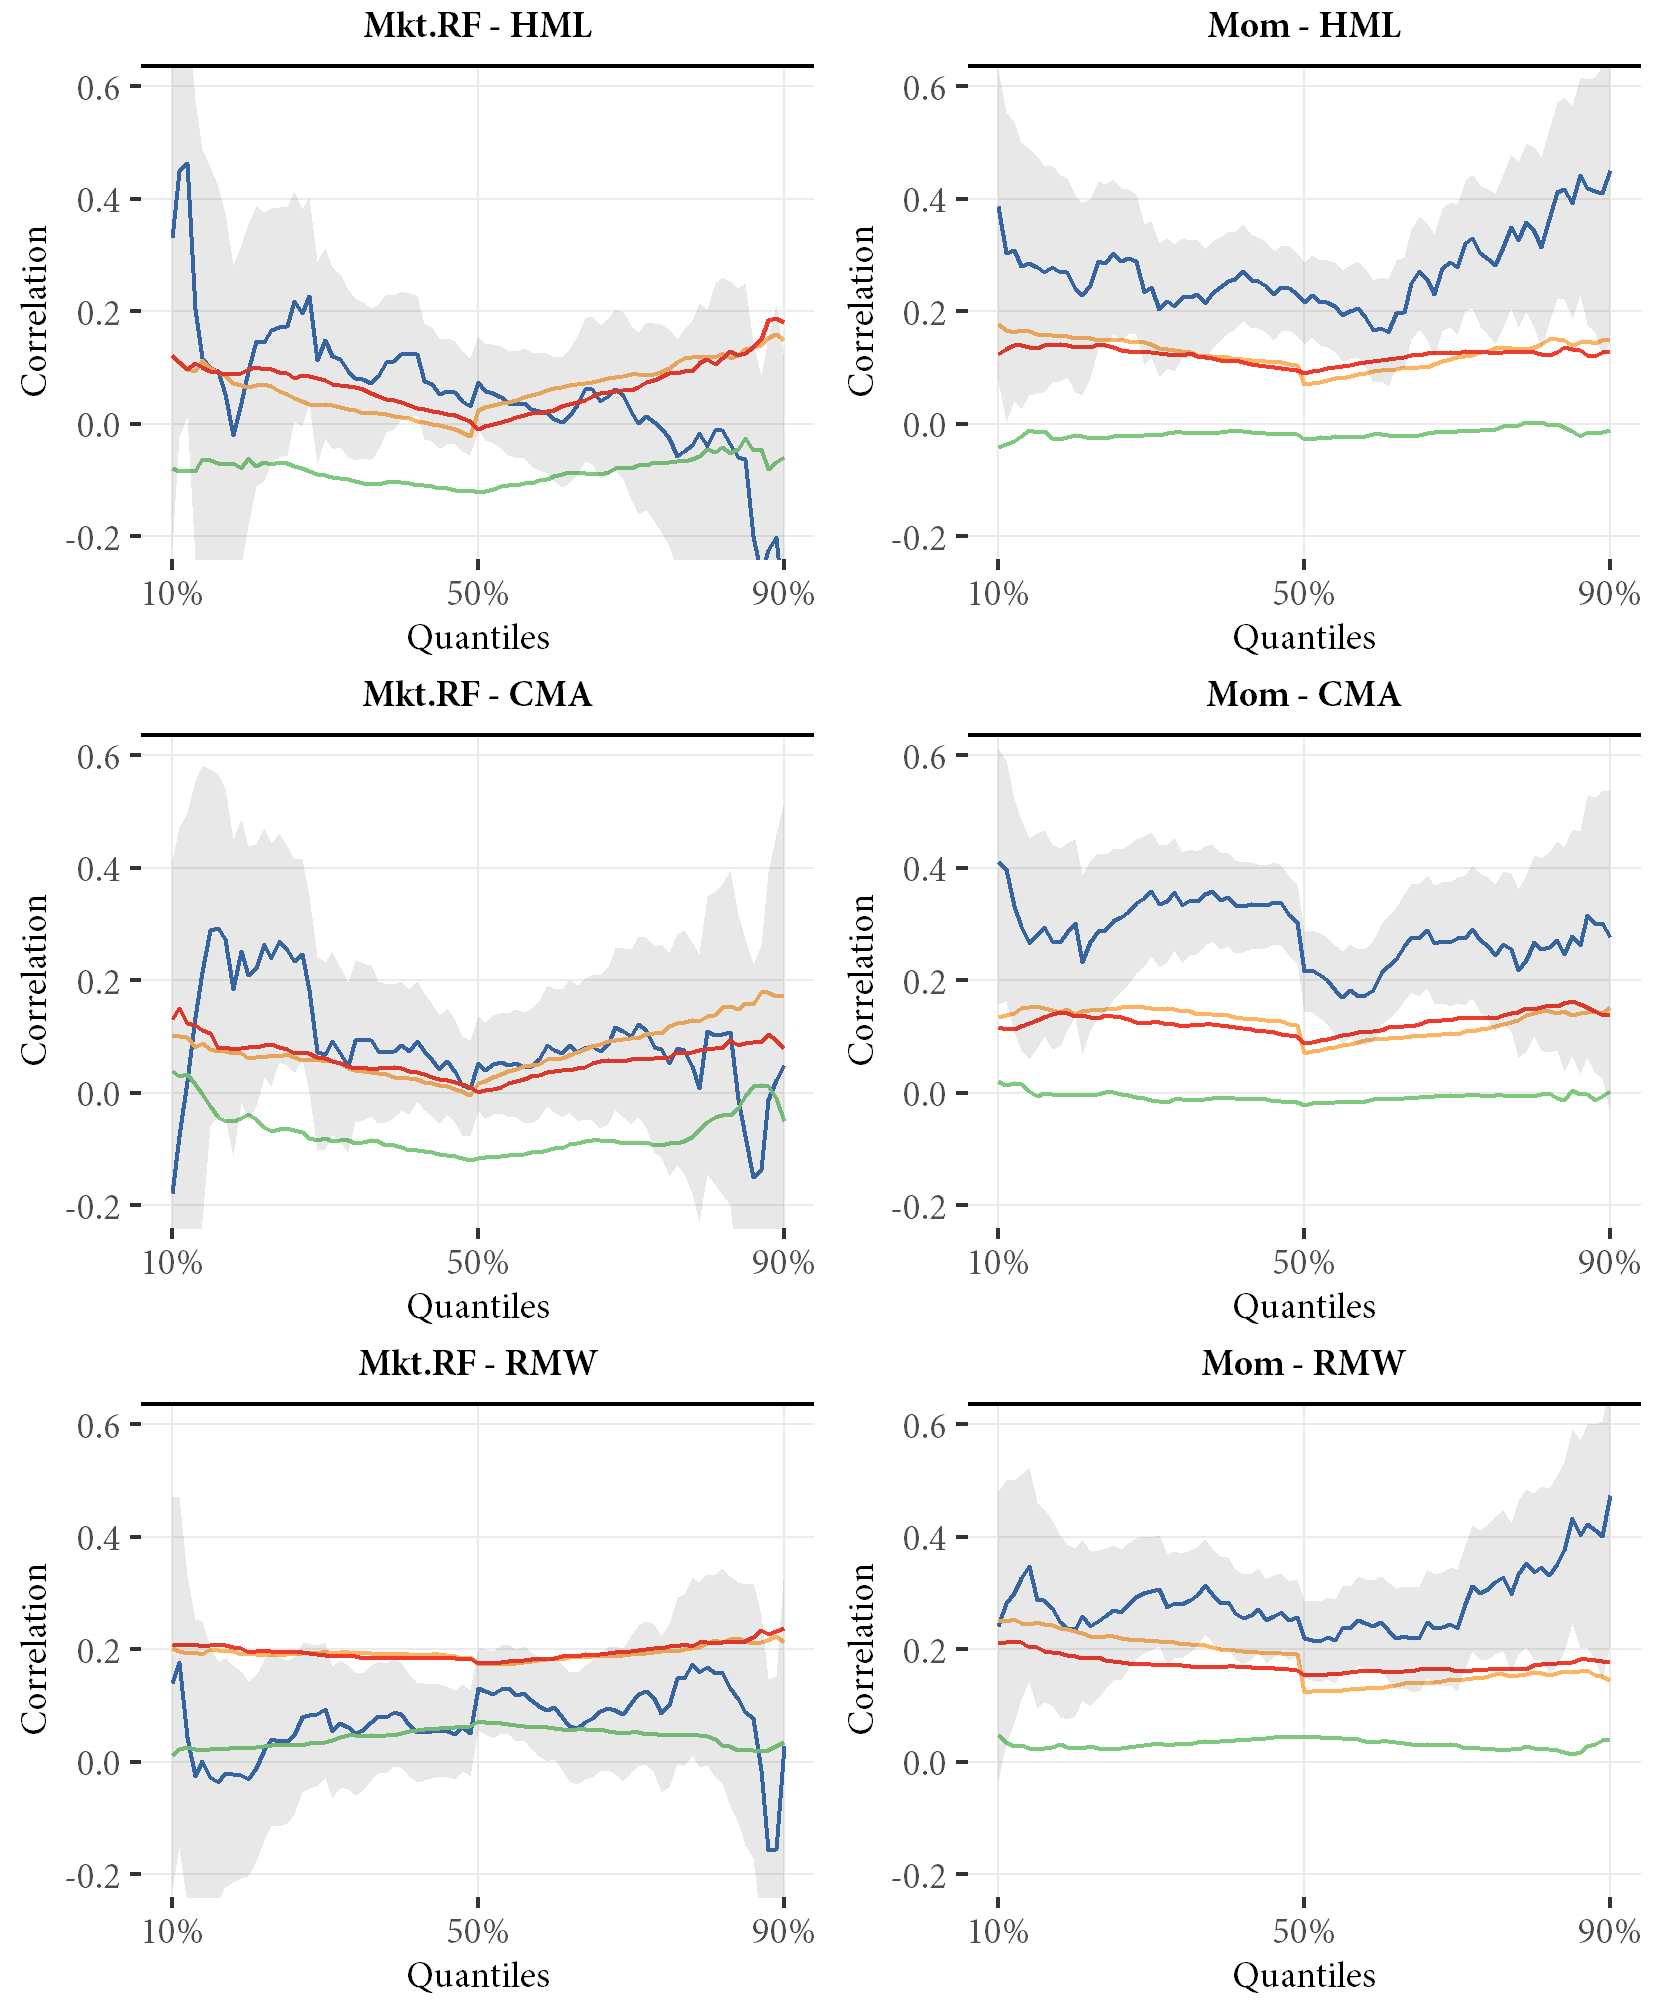
\includegraphics[scale=1]{graphics/threshold_simulated1.png}  
  %\bottomrule
  \vspace{3mm}
  \footnotesize
  ARMA-GARCH threshold correlation plots with 95\% confidence bounds are compared to simulated threshold correlations from the constant copulae with normal, Student's \textit{t} and skewed Student's \textit{t} innovations. 250,000 simulation runs for each. Correlation pairs in graph titles. Weekly data 1963-2016
  \end{minipage}
\end{figure}
\begin{figure}[htbp]
  \caption{Threshold correlations -- comparison of ARMA-GARCH residuals and simulated residuals from constant copulae. Page 2/2}
  \label{fig:threshold_simulated2}
  %\toprule
  \centering
  \begin{minipage}{\textwidth}
  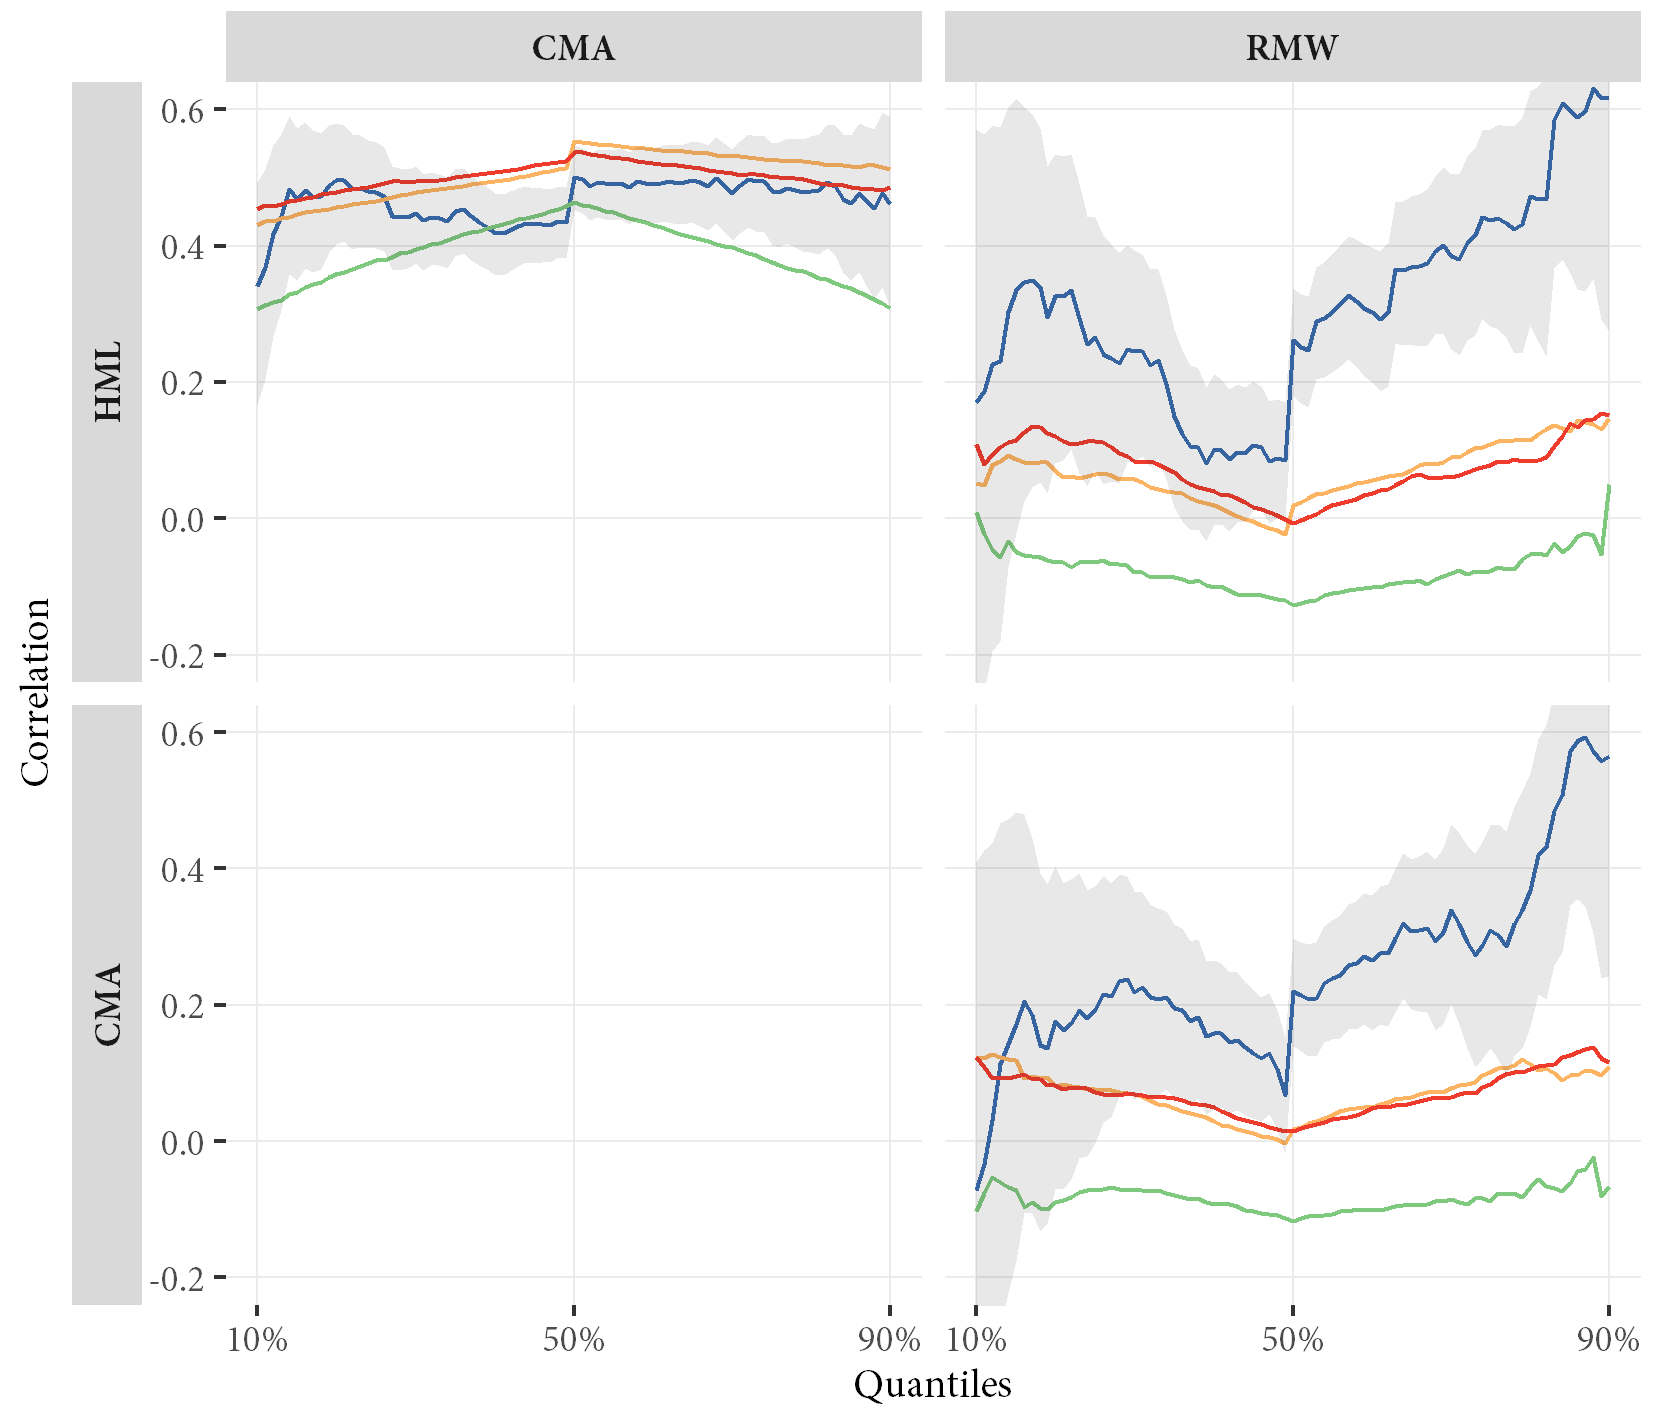
\includegraphics[scale=1]{graphics/threshold_simulated2.png}  
  %\bottomrule
  \vspace{3mm}
  \footnotesize
  ARMA-GARCH threshold correlation plots with 95\% confidence bounds are compared to simulated threshold correlations from the constant copulae with normal, Student's \textit{t} and skewed Student's \textit{t} innovations. 250,000 simulation runs for each. Correlation pairs in graph titles. Weekly data 1963-2016
  \end{minipage}
\end{figure}
% talk
In each plot, we present the empirical threshold correlation with its associated 95\% confidence bound, along with three copula models: the standard normal copula, the Student's \textit{t} copula and the skewed Student's \textit{t}.

First, we note that for most factors, the normal copula is the farthest away from generating threshold correlations that correspond to the empirical distribution around the median. More specifically, it seems to underestimate the threshold correlation, i.e. not generate sufficient tail dependence. The Student's \textit{t} and skewed Student's \textit{t} copulae better capture the threshold correlations, as the fatter tails of the Student's \textit{t} distribution allows for tail dependence. For example, note how the normal copula generates negative threshold correlations for both the Mom - HML and RMW - HML asset pairs, while the Student's \textit{t} based copulae are much closer to the higher values in the data. On the other hand, the Student's \textit{t} based copulae sometimes seem to overshoot the empirical threshold correlation, as in the Mkt-RF - RMW asset pair.

Second, we find that although the skewed Student's \textit{t} does generate some asymmetry around the mean, which can be seen most clearly for the Mom - RMW and RMW - HML asset pairs, the asymmetry is far too weak to be an accurate description of the data. 

In conclusion, threshold correlation comparison between empirical and simulated data shows the limitations of our copula approach. Although the copulae are flexible and can express tail dependence, which is a clear improvement to no tail dependence at all, it does not overlap very well with the data. For example, the Student's \textit{t} copula only has one degree of freedom parameter that controls the fatness of tails, and the skewed Student's \textit{t} copula only has one skewness parameter for each series. This imposes limits on how strongly the model can express fat tails or asymmetries between factors A and B and simultaneously express other fat tails or asymmetries (or lack thereof) between factors A and C. For a collection of six factors with heterogenous dependence, this is even harder. This is a clear limitation of the quite parsimonious copula approach, and will be discussed further in the concluding section. Although imperfect, the copula modeling of tail dependence could constitute a significant improvement to alternatives, especially in the field of risk management, where understanding of tail events is paramount.

% TABLES NEED TO BE MODIFIED IN THE FOLLOWING WAYS
% 1) Change {tabular} to {tabularx}{\textwidth} and make leftmost column an X column
%     and change top and bottom \hline to \toprule \bottomrule
%
% paste the following at start but before & \multicolumn
%
% \begin{tabularx}{\textwidth}{@{\extracolsep{5pt}} X D{.}{.}{-3} D{.}{.}{-3} D{.}{.}{-3} } 
% \\[-1.8ex] \midrule
% \\[-1.8ex] 
%
% paste the following at end after R2 row but before Note row
% \bottomrule \\[-1.8ex] 
%
% 2) Change the variable names to greeks
% 3) Change specification names if needed
% 4) Change R2 to LLH and add similar lines for Ljung-Box and ARCH-LM
% 5) Add label and caption
% 6) Paste this to get table heading description
% 7) Copy table heading tabularx footnote size text
%
% \begin{tabularx}{\textwidth}{X}
% \\[-1.8ex]\toprule
%\\[-1.8ex] 
% text goes here
% \end{tabularx}
%
% 6) Copy the whole table, only change caption, label, factor/spec labels and (1)-(3) to (4)-(6)
% Table created by stargazer v.5.2 by Marek Hlavac, Harvard University. E-mail: hlavac at fas.harvard.edu
% Date and time: ons, okt 12, 2016 - 12:37:02
% Requires LaTeX packages: dcolumn 
\begin{table}[!htbpp] \centering 
  \caption{Copula results: Constant specifications} 
  \label{tab:copula_estimates_constant} 
\begin{tabularx}{\textwidth}{X}
  \\[-1.8ex]\toprule
  \\[-1.8ex] 
  \footnotesize Parameter estimates from constant copula models based on uniform residuals from ARMA-GARCH models. Stationary bootstrap standard errors in parentheses, following \textcite{PolitisRomano1994}. Copula parameters: $\nu$ is the degree of freedom, $\gamma$ is the vector of skewness parameters, $\alpha, \beta$ are the shock loading and autoregressive loading of the \textit{c}DCC process. All data 1963-07-05 - 2016-07-01. 
\end{tabularx}
\begin{tabularx}{\textwidth}{@{\extracolsep{5pt}} X D{.}{.}{-3} D{.}{.}{-3} D{.}{.}{-3} } 
  \\[-1.8ex]\midrule
  \\[-1.8ex] 
   & \multicolumn{3}{c}{Constant copula models} \\ 
  \cline{2-4} 
  \\[-1.8ex] & \multicolumn{1}{c}{(1)} & \multicolumn{1}{c}{(2)} & \multicolumn{1}{c}{(3)}\\ 
  \\[-1.8ex] & \multicolumn{1}{c}{Gaussian} & \multicolumn{1}{c}{Student-\textit{t}} & \multicolumn{1}{c}{Skewed Student-\textit{t}}\\ 
  \hline \\[-1.8ex] 
 $\nu$ &  & 6.625 & 6.671 \\ 
  &  & () & () \\ 
  & & & \\ 
 $\gamma_{Mkt.RF}$ &  &  & -0.057 \\ 
  &  &  & () \\ 
  & & & \\ 
 $\gamma_{SMB}$ &  &  & -0.103 \\ 
  &  &  & () \\ 
  & & & \\ 
 $\gamma_{Mom}$ &  &  & -0.202 \\ 
  &  &  & () \\ 
  & & & \\ 
 $\gamma_{HML}$ &  &  & 0.103 \\ 
  &  &  & () \\ 
  & & & \\ 
 $\gamma_{CMA}$ &  &  & 0.076 \\ 
  &  &  & () \\ 
  & & & \\ 
 $\gamma_{RMW}$ &  &  & 0.021 \\ 
  &  &  & () \\ 
  & & & \\ 
\hline \\[-1.8ex] 
Observations & \multicolumn{1}{c}{2,766} & \multicolumn{1}{c}{2,766} & \multicolumn{1}{c}{2,766} \\ 
LLH & \multicolumn{1}{c}{1,169} & \multicolumn{1}{c}{1,556} & \multicolumn{1}{c}{1,573} \\ 
No. parameters & \multicolumn{1}{c}{15} & \multicolumn{1}{c}{16} & \multicolumn{1}{c}{22} \\ 
BIC & \multicolumn{1}{c}{-2,220} & \multicolumn{1}{c}{-2,985} & \multicolumn{1}{c}{-2,971} \\ 
Correlation $(Q)$ persistence $(\alpha+\beta)$ & \multicolumn{1}{c}{N/A} & \multicolumn{1}{c}{N/A} & \multicolumn{1}{c}{N/A} \\ 
\bottomrule \\[-1.8ex] 
\textit{Note:}  & \multicolumn{3}{c}{$^{*}$p$<$0.1; $^{**}$p$<$0.05; $^{***}$p$<$0.01} \\ 
\end{tabularx} 
\end{table} 


\subsection{Copula results with dynamic correlations}
%\label
% still haven't captured dynamic, lets do this now
% diagnostics of fit
% why we prefer symmetric t
% correlation patterns over time in-sample graph looks very much like the data rolling
% Table created by stargazer v.5.2 by Marek Hlavac, Harvard University. E-mail: hlavac at fas.harvard.edu
% Date and time: ons, okt 12, 2016 - 12:37:02
% Requires LaTeX packages: dcolumn 
\begin{table}[!htbpp] \centering 
  \caption{Copula results: \textit{c}DCC specifications} 
  \label{tab:copula_estimates_dynamic} 
\begin{tabularx}{\textwidth}{X}
\\[-1.8ex]\toprule
\\[-1.8ex] 
\footnotesize Parameter estimates from dynamic copula models based on uniform residuals from ARMA-GARCH models. Stationary bootstrap standard errors in parentheses, following \textcite{PolitisRomano1994}. Copula parameters: $\nu$ is the degree of freedom, $\gamma$ is the vector of skewness parameters, $\alpha, \beta$ are the shock loading and autoregressive loading of the \textit{c}DCC process. All data 1963-07-05 - 2016-07-01. 
\end{tabularx}
\begin{tabularx}{\textwidth}{@{\extracolsep{5pt}} X D{.}{.}{-3} D{.}{.}{-3} D{.}{.}{-3} } 
\\[-1.8ex]\midrule
\\[-1.8ex] 
 & \multicolumn{3}{c}{Dynamic copula models} \\ 
\cline{2-4} 
\\[-1.8ex] & \multicolumn{1}{c}{(4)} & \multicolumn{1}{c}{(5)} & \multicolumn{1}{c}{(6)}\\ 
\\[-1.8ex] & \multicolumn{1}{c}{Gaussian} & \multicolumn{1}{c}{Student-\textit{t}} & \multicolumn{1}{c}{Skewed Student-\textit{t}}\\ 
\hline \\[-1.8ex] 
 $\nu$ &  & 11.936 & 11.881^{***} \\ 
  &  & () & (1.064) \\ 
  & & & \\ 
 $\gamma_{Mkt.RF}$ &  &  & -0.078 \\ 
  &  &  & (0.054) \\ 
  & & & \\ 
 $\gamma_{SMB}$ &  &  & -0.175^{**} \\ 
  &  &  & (0.077) \\ 
  & & & \\ 
 $\gamma_{Mom}$ &  &  & -0.145^{*} \\ 
  &  &  & (0.073) \\ 
  & & & \\ 
 $\gamma_{HML}$ &  &  & 0.083 \\ 
  &  &  & (0.058) \\ 
  & & & \\   
 $\gamma_{CMA}$ &  &  & 0.001 \\ 
  &  &  & (0.063) \\ 
  & & & \\ 
 $\gamma_{RMW}$ &  &  & 0.095 \\ 
  &  &  & (0.061) \\ 
  & & & \\ 
 $\alpha$ & 0.065 & 0.068 & 0.068^{***} \\ 
  & () & () & (0.007) \\ 
  & & & \\ 
 $\beta$ & 0.915 & 0.913 & 0.913^{***} \\ 
  & () & () & (0.011) \\ 
  & & & \\ 
\hline \\[-1.8ex] 
Observations & \multicolumn{1}{c}{2,766} & \multicolumn{1}{c}{2,766} & \multicolumn{1}{c}{2,766} \\ 
LLH & \multicolumn{1}{c}{2,791} & \multicolumn{1}{c}{2,978} & \multicolumn{1}{c}{2,989} \\ 
No. parameters & \multicolumn{1}{c}{17} & \multicolumn{1}{c}{18} & \multicolumn{1}{c}{24} \\ 
BIC & \multicolumn{1}{c}{-5,447} & \multicolumn{1}{c}{-5,813} & \multicolumn{1}{c}{-5,788} \\ 
Correlation $(Q)$ persistence $(\alpha+\beta)$ & \multicolumn{1}{c}{0.981} & \multicolumn{1}{c}{0.981} & \multicolumn{1}{c}{0.981} \\ 
\bottomrule \\[-1.8ex] 
\textit{Note:}  & \multicolumn{3}{c}{$^{*}$p$<$0.1; $^{**}$p$<$0.05; $^{***}$p$<$0.01} \\ 
\end{tabularx} 
\end{table} 
